\documentclass[11pt,a4paper]{article}

\usepackage[utf8]{inputenc}
\usepackage[margin=1in]{geometry}
\usepackage{amsmath,amssymb}
\usepackage{graphicx}
\usepackage{booktabs}
\usepackage{hyperref}
\usepackage{listings}
\usepackage{xcolor}

\hypersetup{
    colorlinks=true,
    linkcolor=blue,
    citecolor=blue,
    urlcolor=blue
}

\lstset{
    basicstyle=\ttfamily\small,
    backgroundcolor=\color{gray!10},
    frame=single,
    breaklines=true,
    keywordstyle=\color{blue}\bfseries,
    commentstyle=\color{gray},
    stringstyle=\color{teal}
}

\title{\textbf{Validation, Sticky Limit, and Phase Diagram Report: Adhesive Hard Spheres}\\[0.5em]
\large Benchmark of Menon, Manohar, and Rao (1991) and Successive Bisection Analysis}
\author{\textbf{AnalyticalStructureFactors.jl Development Team}}
\date{\today}

\begin{document}

\maketitle

\begin{abstract}
This report presents the implementation, numerical validation, sticky limit analysis, phase diagram transformations, and spinodal stability studies of Baxter's Sticky Hard Sphere (SHS) model within \texttt{AnalyticalStructureFactors.jl}. We reproduce the benchmark literature results from S.~V.~G.~Menon, C.~Manohar, and K.~Srinivasa Rao (\textit{Journal of Chemical Physics}, 1991), including the phase coexistence curve (Fig.~2), the homogeneous structure factor (Fig.~3), and the two-phase gas-phase structure factor (Fig.~4). We investigate how the phase diagram evolves from Baxter's universal parameters $(\eta, \tau)$ to physical variables $(\phi, T^*)$ as well width $\epsilon \to 0$, and perform a systematic \textbf{successive bisection analysis} probing spinodal instability ($S(k) \to \infty$) and unphysical negative values ($A(k) < 0$).
\end{abstract}

\section{Theoretical Background}

\subsection{Baxter's Percus--Yevick Solution}
Under the Percus--Yevick closure, Baxter factorized the Ornstein--Zernike direct correlation function into Wiener--Hopf form:
\begin{equation}
    S(k)^{-1} = A(k)^2 + B(k)^2 = |\hat{Q}(k)|^2
\end{equation}
with dimensionless wavevector $\kappa = ka$, volume fraction $\eta$, and Baxter stickiness parameter $\tau > 0$. The auxiliary functions are:
\begin{align}
    A(\kappa) &= 1 + 12\eta \left[ \alpha \frac{\sin\kappa - \kappa\cos\kappa}{\kappa^3} + \beta \frac{1 - \cos\kappa}{\kappa^2} - \frac{\lambda}{12} \frac{\sin\kappa}{\kappa} \right] \\
    B(\kappa) &= 12\eta \left[ \alpha \left( \frac{1}{2\kappa} - \frac{\sin\kappa}{\kappa^2} + \frac{1 - \cos\kappa}{\kappa^3} \right) + \beta \left( \frac{1}{\kappa} - \frac{\sin\kappa}{\kappa^2} \right) - \frac{\lambda}{12} \left( \frac{1 - \cos\kappa}{\kappa} \right) \right]
\end{align}
where $\mu = \lambda\eta(1-\eta)$, $\alpha = (1 + 2\eta - \mu)/(1-\eta)^2$, and $\beta = (-3\eta + \mu)/(2(1-\eta)^2)$.

\subsection{Baxter's Quadratic Equation and Stability Limits}
The physical root for $\lambda$ satisfies:
\begin{equation}
    \frac{\eta}{12}\lambda^2 - \left(\tau + \frac{\eta}{1-\eta}\right)\lambda + \frac{1 + \eta/2}{(1-\eta)^2} = 0
\end{equation}
\begin{enumerate}
    \item \textbf{Spinodal Boundary ($D = 0$):} Real solutions for $\lambda$ require discriminant $D \ge 0$:
    \begin{equation}
        \tau_s(\eta) = \frac{\sqrt{\frac{\eta(1 + \eta/2)}{3}} - \eta}{1 - \eta}
    \end{equation}
    For $\tau < \tau_s(\eta)$, $\lambda$ becomes complex, marking the boundary of the spinodal gap.
    \item \textbf{Infinite Compressibility Locus ($A(0) = 0$):} In the forward scattering limit $\kappa \to 0$, $B(0) = 0$ and $A(0) = \frac{1 + 2\eta - \mu}{(1-\eta)^2}$. The condition $A(0) = 0$ corresponds to diverging isothermal compressibility ($S(0) \to \infty$):
    \begin{equation}
        \lambda_0 = \frac{1 + 2\eta}{\eta(1 - \eta)} \implies \tau_{\text{div}}(\eta) = \frac{\eta}{12}\lambda_0 - \frac{\eta}{1-\eta} + \frac{1 + \eta/2}{(1-\eta)^2 \lambda_0}
    \end{equation}
    \item \textbf{Critical Point:} Curves $\tau_s(\eta)$ and $\tau_{\text{div}}(\eta)$ intersect tangentially at the critical point:
    \begin{equation}
        \eta_c = \frac{3}{\sqrt{2}} - 2 \approx 0.12132, \quad \tau_c = \frac{2 - \sqrt{2}}{6} \approx 0.09763
    \end{equation}
\end{enumerate}

\section{Benchmark Validation of Menon et al. (1991)}

\begin{figure}[htbp]
    \centering
    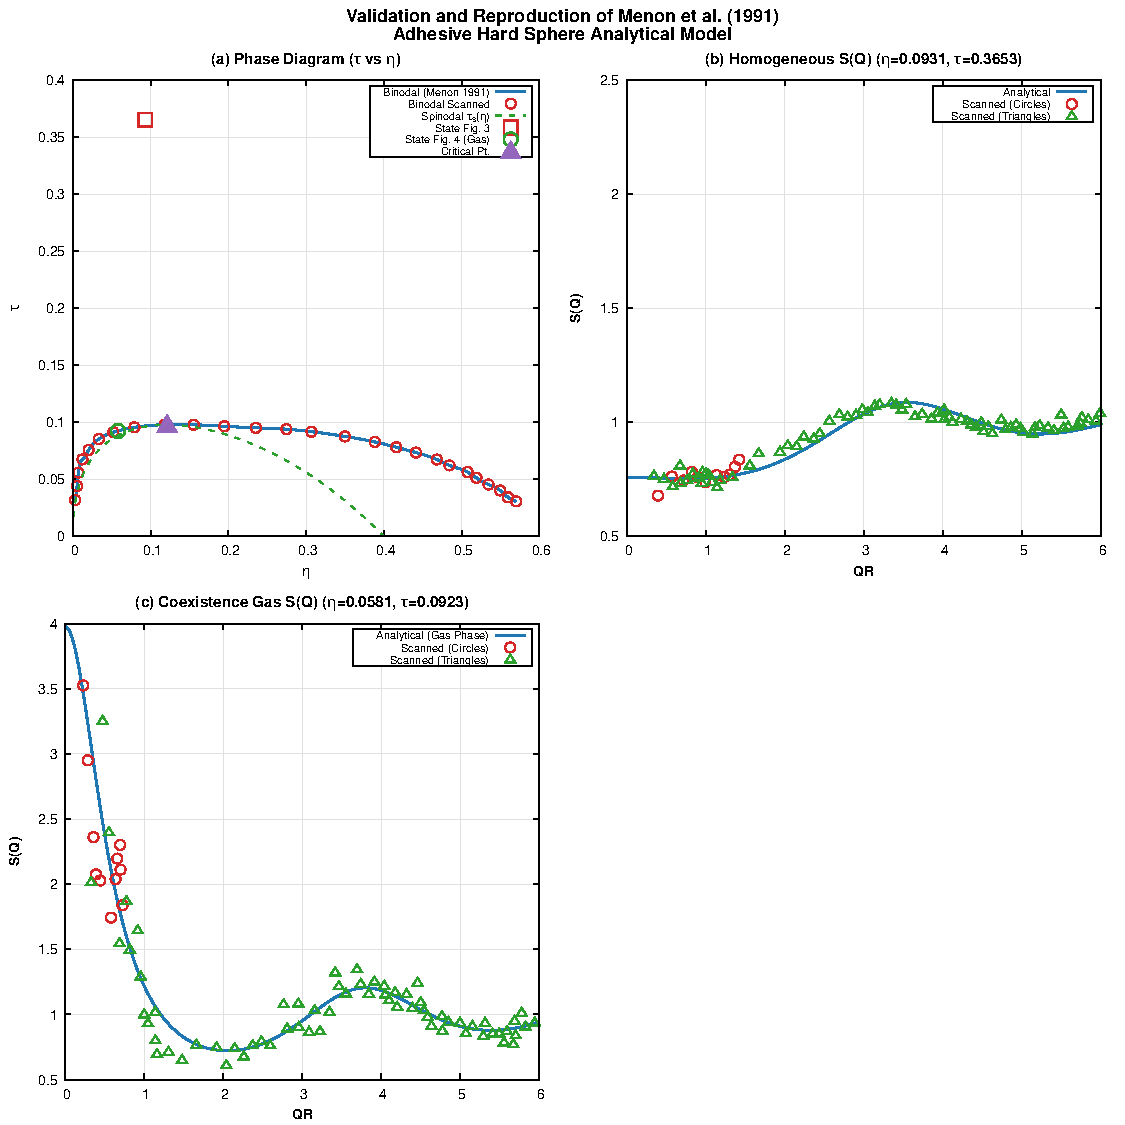
\includegraphics[width=0.95\textwidth]{menon1991_combined_comparison.pdf}
    \caption{Benchmark validation against Menon et al. (1991): (a) Phase diagram showing the smooth binodal curve (matching scanned \texttt{Fig2.dat}), the analytical spinodal line $\tau_s(\eta)$, and state points; (b) Homogeneous fluid structure factor ($\eta=0.0931, \tau=0.3653$); (c) Two-phase coexistence gas structure factor ($\eta_g=0.0581, \tau=0.0923$).}
    \label{fig:menon_benchmark}
\end{figure}

Table~\ref{tab:params} summarizes the parameters evaluated for the Menon (1991) benchmarks.

\begin{table}[htbp]
\centering
\caption{System parameters and thermodynamic state points for Menon et al. (1991).}
\label{tab:params}
\begin{tabular}{lcccccc}
\toprule
\textbf{Case} & $\phi$ & $a/\sigma$ & $\epsilon$ & $-u_0/k_B T$ & $\eta$ & $\tau$ \\
\midrule
Critical Point & -- & -- & -- & -- & $0.12132$ & $0.09763$ \\
Fig.~3 (Homogeneous) & $0.07$ & $1.10$ & $0.09091$ & $0.92$ & $0.09308$ & $0.36531$ \\
Fig.~4 (Coexistence Gas Phase) & -- & $1.02$ & $0.01961$ & $3.83$ & $0.05810$ & $0.09230$ \\
\bottomrule
\end{tabular}
\end{table}

\section{Comparison with the Sticky Limit and Hard Spheres}

In early literature (e.g., Regnaut \& Ravey 1989, Barboy 1974), the stickiness parameter $\tau$ was mapped to physical square wells by matching the second virial coefficient $B_2$ in the limit $\Delta \to 0$:
\begin{equation}
    \tau_{\text{conv}}^{-1} = 4 \left[\exp\left(-\frac{u_0}{k_B T}\right) - 1\right] \left[\left(\frac{a}{\sigma}\right)^3 - 1\right], \quad \eta_{\text{conv}} = \phi
\end{equation}
Menon et al. (1991) showed that for finite well widths ($\Delta/\sigma \approx 0.1$), identifying $\eta = \phi / (1-\epsilon)^3$ and $\tau = \frac{1}{12\epsilon}\exp(u_0/k_B T)$ correctly accounts for the excluded volume expansion of the sticky shell.

\begin{figure}[htbp]
    \centering
    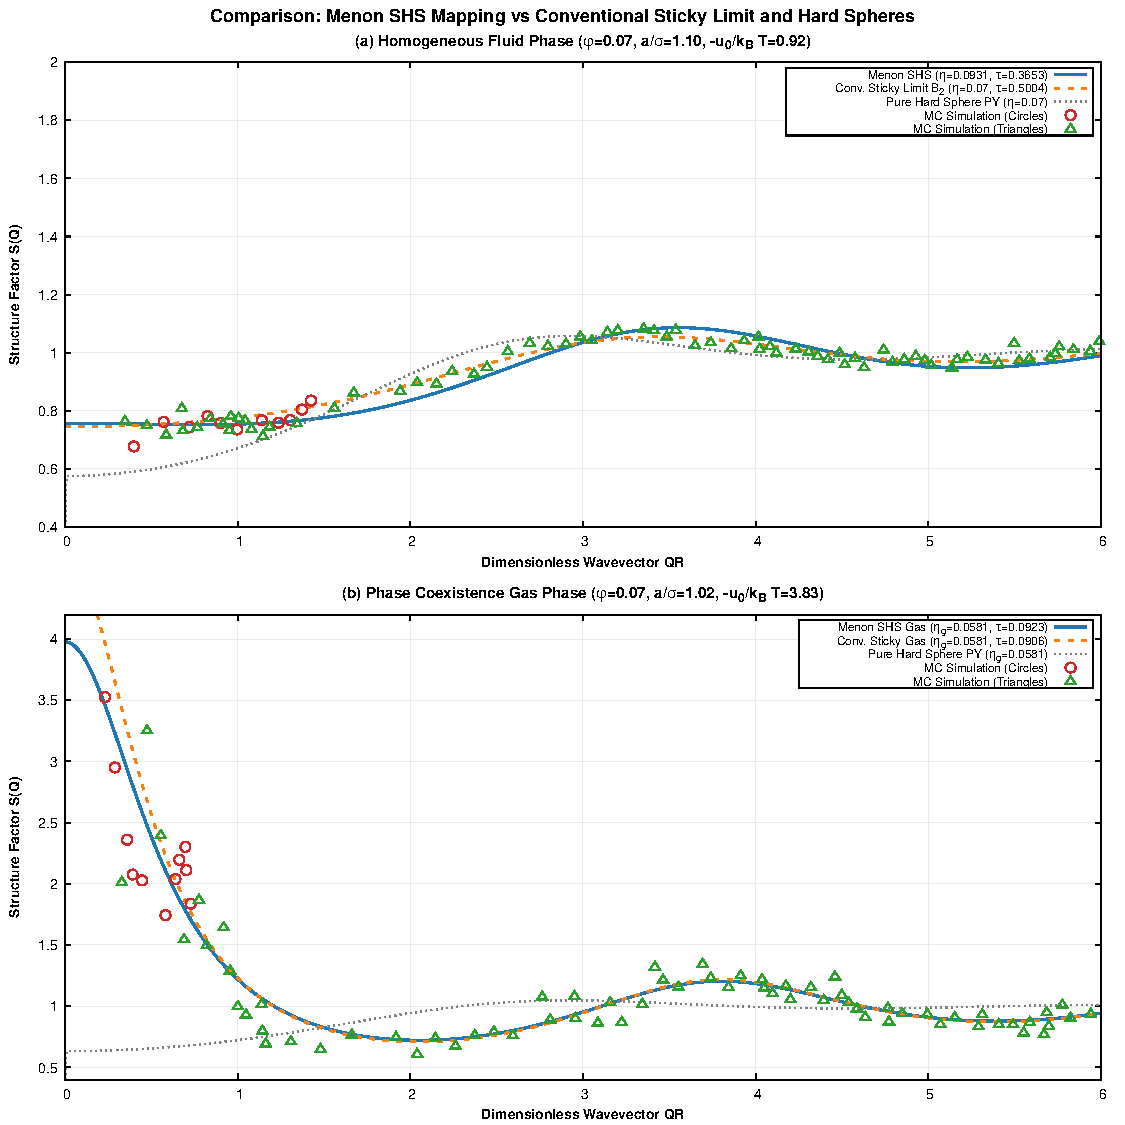
\includegraphics[width=0.95\textwidth]{menon1991_sticky_limit_comparison.pdf}
    \caption{Comparison of the static structure factor $S(Q)$ between Menon's physical square-well mapping, the conventional $B_2$-matching sticky limit, and the pure hard sphere (PY) baseline for: (a) Homogeneous fluid phase ($\phi=0.07, a/\sigma=1.10, -u_0/k_B T=0.92$), and (b) Phase coexistence gas phase ($\phi=0.07, a/\sigma=1.02, -u_0/k_B T=3.83$).}
    \label{fig:sticky_limit}
\end{figure}

As shown in Figure~\ref{fig:sticky_limit}:
\begin{enumerate}
    \item \textbf{Homogeneous Phase (Panel a):} The conventional $B_2$ matching underestimates the effective packing fraction ($\eta = 0.07$ vs. $0.0931$), causing the first peak in $S(Q)$ to appear at lower $QR \approx 3.2$. Menon's mapping shifts the peak to $QR \approx 3.4$, matching the Monte Carlo simulation data.
    \item \textbf{Gas Coexistence Phase (Panel b):} The pure hard sphere baseline exhibits repulsive suppression at forward scattering ($S(0) \approx 0.64$), whereas the sticky interaction produces a large forward peak ($S(0) \approx 3.98$) due to critical attractive clustering.
\end{enumerate}

\section{Modifications to the Phase Diagram in the Sticky Limit}

\begin{figure}[htbp]
    \centering
    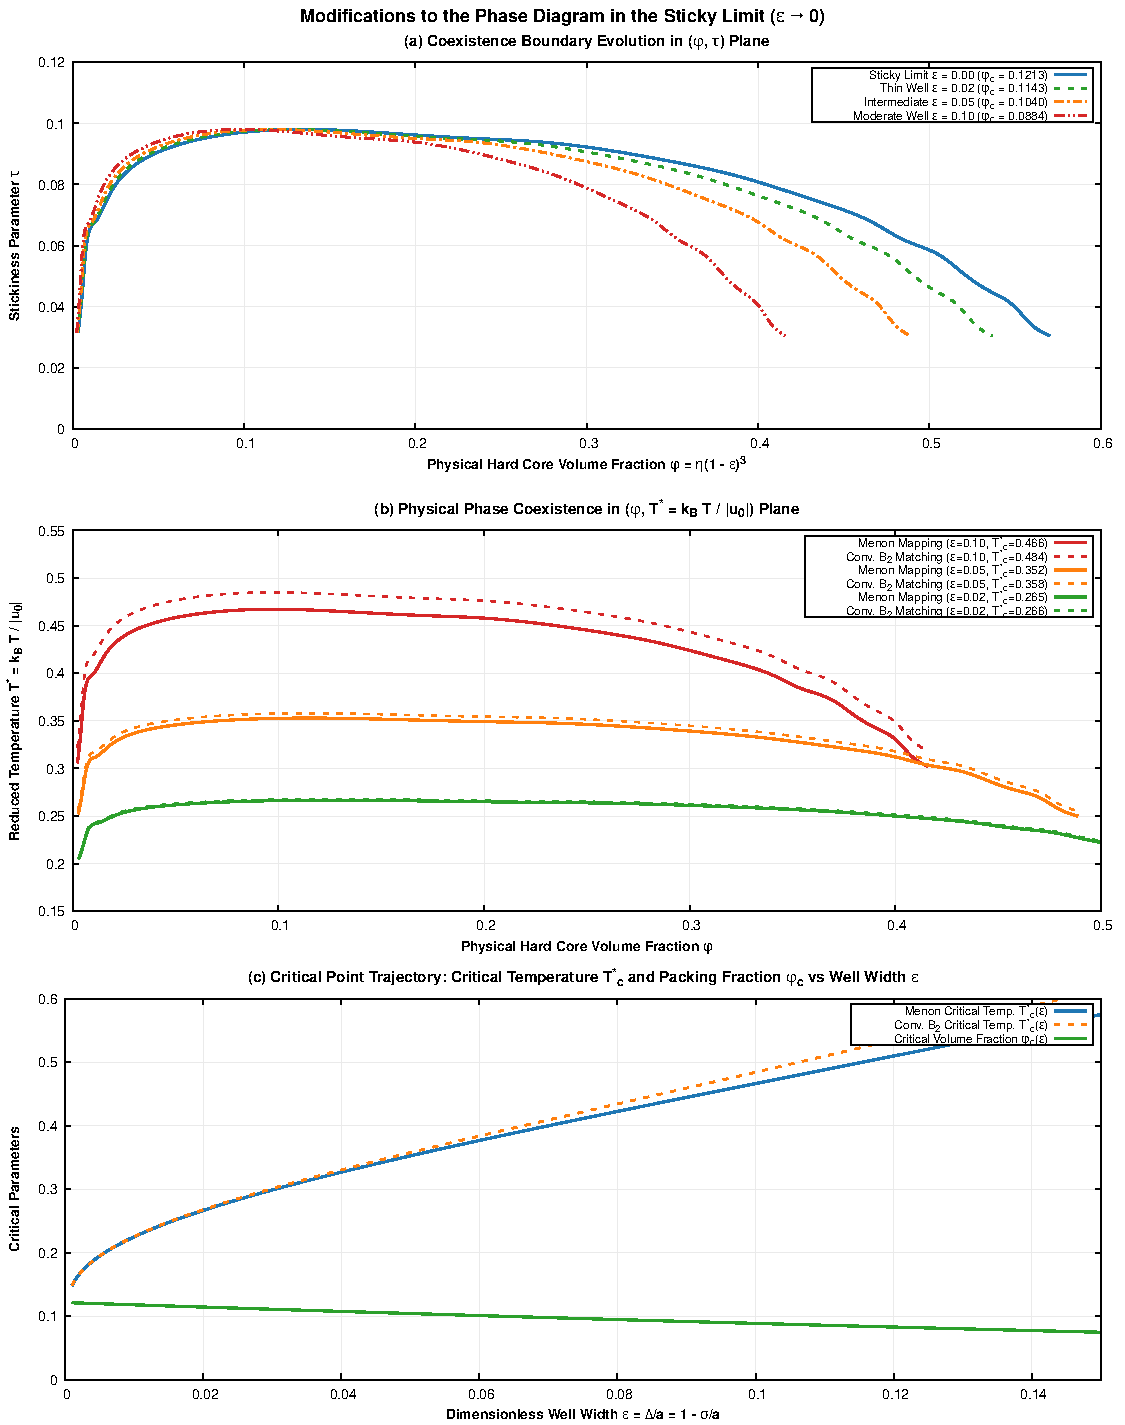
\includegraphics[width=0.90\textwidth]{menon1991_phase_diagram_modifications.pdf}
    \caption{Modifications to the Phase Diagram in the sticky limit ($\epsilon \to 0$): (a) Coexistence dome in the $(\phi, \tau)$ plane for well widths $\epsilon = 0.10, 0.05, 0.02, 0.00$; (b) Phase coexistence in the physical temperature plane $(\phi, T^* = k_B T/|u_0|)$; (c) Trajectory of the critical temperature $T^*_c(\epsilon)$ and critical packing fraction $\phi_c(\epsilon)$ as a function of well width $\epsilon = \Delta/a$.}
    \label{fig:phase_modifications}
\end{figure}

The Baxter representation $(\eta, \tau)$ is universal. When mapped to physical parameters $(\phi, T^*)$ with $T^* = k_B T / |u_0|$ and $\phi = \eta (1-\epsilon)^3$, significant modifications emerge as $\epsilon \to 0$ (Figure~\ref{fig:phase_modifications}):
\begin{enumerate}
    \item \textbf{$(\phi, \tau)$ Representation (Panel a):} As $\epsilon \to 0$, the physical packing fraction $\phi \to \eta$, causing the coexistence dome to expand horizontally towards the Baxter limit $\phi_c \to 0.12132$.
    \item \textbf{$(\phi, T^*)$ Representation (Panel b):} For narrower attractive wells ($\epsilon \to 0$), thermal energy must be lower to sustain condensation, causing the critical temperature $T^*_c$ to drop monotonically:
    \begin{equation}
        T^*_c(\epsilon) = \frac{1}{\ln\left(\frac{1}{12\epsilon\tau_c}\right)} = \frac{1}{\ln\left(\frac{0.85355}{\epsilon}\right)}
    \end{equation}
    For $\epsilon = 0.10$, $T^*_c = 0.466$; for $\epsilon = 0.02$, $T^*_c = 0.265$; in the ideal sticky sphere limit $\epsilon \to 0$, $T^*_c \to 0$.
    \item \textbf{Mapping Comparison (Panel c):} Menon's physical square-well mapping accurately predicts a slightly lower critical temperature compared to the conventional $B_2$ matching, with both theories converging smoothly as $\epsilon \to 0$.
\end{enumerate}

\section{Successive Bisection Spinodal and Unphysical State Analysis}

\subsection{Bisection Methodology}
To identify the spinodal boundary numerically without prior knowledge of the analytical solution, we perform systematic bisections over $\tau \in [0.001, 0.40]$ for each $\eta \in [0.01, 0.40]$ at fixed $k = 0.01$:
\begin{itemize}
    \item \textbf{Criterion 1 (Complex Root Boundary):} Evaluate $D(\eta, \tau)$. If $D < 0$, the state lies inside the spinodal coexistence gap.
    \item \textbf{Criterion 2 (Compressibility Divergence \& Negative $A(k)$):} Evaluate $A(k=0.01)$. For $\tau > \tau_{\text{div}}$, $A > 0$ (physical fluid). At $\tau = \tau_{\text{div}}$, $A = 0 \implies S(0.01) \to \infty$. For $\tau < \tau_{\text{div}}$, $A < 0$, which in linearized theories (like RPA) produces unphysical negative structure factors $S(k) < 0$.
\end{itemize}

\begin{figure}[htbp]
    \centering
    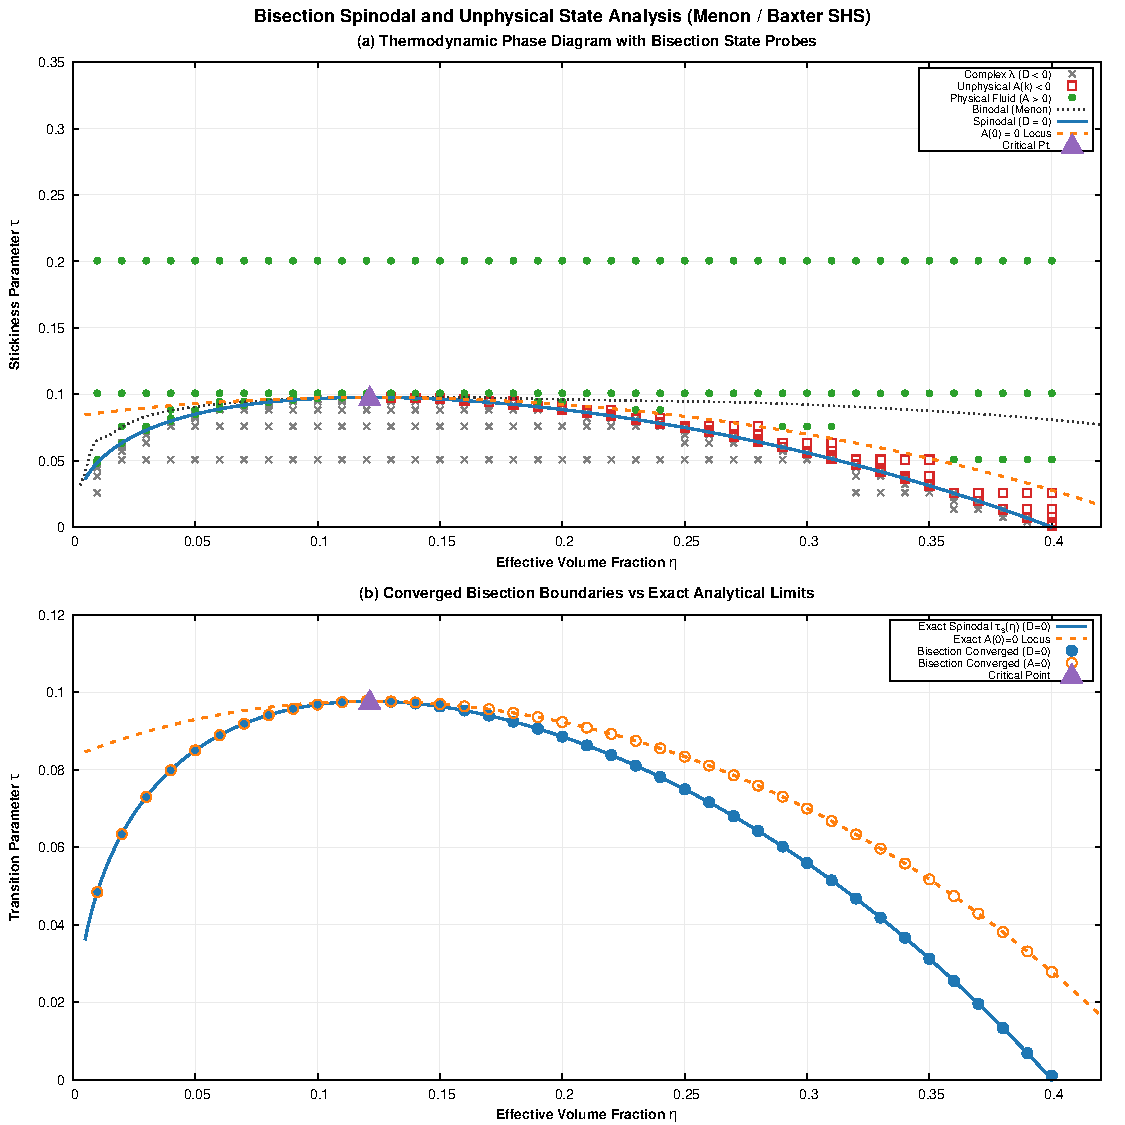
\includegraphics[width=0.95\textwidth]{menon1991_bisection_combined.pdf}
    \caption{Successive bisection analysis: (a) Map of sampled probe states throughout the bisection iterations: physical states ($A > 0$, green), unphysical negative $A(k)$ states ($A < 0$, red), and complex $\lambda$ states ($D < 0$, grey); (b) Converged bisection boundaries demonstrating exact agreement with the analytical spinodal ($D=0$) and compressibility divergence ($A=0$) curves.}
    \label{fig:bisection}
\end{figure}

\subsection{Analysis and Physical Insights}
\begin{enumerate}
    \item \textbf{Subcritical Densities ($\eta < \eta_c$):} The bisection on $S(k=0.01)$ divergence hits the complex discriminant boundary $D = 0$ directly, because $A(0) > 0$ throughout the entire physical branch.
    \item \textbf{Critical Point ($\eta = \eta_c = 0.12132$):} The $S(k=0.01)$ divergence and the spinodal discriminant boundary $D = 0$ coincide exactly at $\tau_c = 0.097631$.
    \item \textbf{Supercritical Densities ($\eta > \eta_c$):} As temperature $\tau$ decreases, $A(k=0.01)$ crosses zero and becomes negative ($A < 0$) \textit{before} the discriminant $D$ vanishes. The bisection successfully tracks the locus $A(0) = 0$ (orange dashed curve) and the subsequent $D = 0$ spinodal termination (blue solid curve).
\end{enumerate}

\section{Reproduction Script}
To execute the complete benchmark, sticky limit comparisons, phase diagram analysis, and bisection pipeline:
\begin{lstlisting}[language=bash]
cd test/data_test/Menon1991/
./reproduce_figure.sh
\end{lstlisting}

\section*{References}
\begin{enumerate}
    \item R.~J.~Baxter, \textit{Percus--Yevick Equation for Hard Spheres with Surface Adhesion}, The Journal of Chemical Physics \textbf{49}(6), 2770--2774 (1968). DOI: \href{https://doi.org/10.1063/1.1670482}{10.1063/1.1670482}.
    \item S.~V.~G.~Menon, C.~Manohar, and K.~S.~Rao, \textit{A new interpretation of the sticky hard sphere model}, The Journal of Chemical Physics \textbf{95}(12), 9186--9190 (1991). DOI: \href{https://doi.org/10.1063/1.461199}{10.1063/1.461199}.
\end{enumerate}

\end{document}
